%%%%%%%%%%%%%%%%%%%%%%%%%% author.tex %%%%%%%%%%%%%%%%%%%%%%%%%
%
% sample root file for your contribution to a "contributed book"
%
% "contributed book"
%
% Use this file as a template for your own input.
%
%%%%%%%%%%%%%%%%%%%%%%%% Springer-Verlag %%%%%%%%%%%%%%%%%%%%%%%%%%


% RECOMMENDED %%%%%%%%%%%%%%%%%%%%%%%%%%%%%%%%%%%%%%%%%%%%%%%%%%%
\documentclass{svmult}

% choose options for [] as required from the list
% in the Reference Guide, Sect. 2.2

\usepackage{amssymb}         % assumes amsmath package installed
\usepackage{amsmath}         % assumes amsmath package installed
\usepackage{makeidx}         % allows index generation
\usepackage{graphicx}        % standard LaTeX graphics tool
                             % when including figure files
\usepackage{multicol}        % used for the two-column index
\usepackage[bottom]{footmisc}% places footnotes at page bottom
% etc.
% see the list of further useful packages
% in the Reference Guide, Sects. 2.3, 3.1-3.3

\makeindex             % used for the subject index
                       % please use the style sprmidx.sty with
                       % your makeindex program

\newcommand{\q}{\mathbf q}
\newcommand{\dq}{\dot {\mathbf q}}
\newcommand{\x}{\mathbf {x}}
\newcommand{\dx}{\dot {\mathbf x}}
\newcommand{\ProofBegin}{{\em Proof.} }
\newcommand{\ProofEnd}{\hfill $\diamondsuit$\\}

\newtheorem{fact}[theorem]{Proposition}
%%%%%%%%%%%%%%%%%%%%%%%%%%%%%%%%%%%%%%%%%%%%%%%%%%%%%%%%%%%%%%%%%%%%%

\begin{document}

\title{Exploiting Motor Modules in Modular Contexts}
% Use \titlerunning{Short Title} for an abbreviated version of
% your contribution title if the original one is too long
\author{Francesco Nori\inst{1}\and
Giorgio Metta\inst{1,2} \and Giulio Sandini\inst{1}}
% Use \authorrunning{Short Title} for an abbreviated version of
% your contribution title if the original one is too long
\institute{Italian Institute of Technology, via Morego 30,
16163 Genova
\texttt{francesco.nori@iit.it, giorgio.metta@iit.it, giulio.sandini@iit.it}
\and University of Genoa, Department of Communication 
Computer and System Sciences, Viale F. Causa 13,  16145
Genoa, Italy}
%
% Use the package "url.sty" to avoid
% problems with special characters
% used in your e-mail or web address
%
\maketitle

\abstract{Recently there has been a growing interest in modeling
motor control systems with modular structures. Such control
structures have many interesting properties, which have been
described in recent studies. This chapter focuses on some properties which
are related to the fact that specific set of contexts can themselves
be modular. Specifically, it shows that the adaptation of a
modular control structure can be guided by the modularity of
contexts, by means of interpreting the current unexperienced context
as the combination of previously experienced contexts.}
%% \title, \author and \abstract MUST be specified before \maketitle.

\section{Introduction}

Humans exhibit a broad repertoire of motor capabilities which can be
performed in a wide range of different environments and situations.
From the point of view of control theory, the problem of dealing
with different environmental situations is nontrivial and requires
significant adaptive capabilities. Even the simple movement of
lifting up an object, depends on many variables, both {\em internal
and external} to the body.
Examples of internal variables
are the state of the arm (e.g. joint angles and angular velocities)
and its dynamic parameters (e.g. masses, moments of inertia, etc.).
However, when interacting with the environment, motor commands need
to be adapted also to some {\em external variables}
which describe the interaction environment (e.g. geometrical and 
dynamical parameters of lifted objects).
All these variables define what is generally called the context of
the movement. As the context of the movement alters the input-output
relationship of the controlled system, the motor command must be
tailored so as to take into account the current context. In everyday
life, humans interact with multiple different environments and their
possible combinations. Therefore, a fundamental question in motor
control concerns how the control system robustly adapts to a continuously
changing operating context.

The adaptation of the motor control system to a continuously 
changing environment is a complex task. Noticeably, the dimensionality
of the context space grows exponentially with the number 
of alternatives/variables used to describe the context itself.
Therefore, this {\em curse of dimensionality} rules out any 
brute force approach for solving the context adaptation problem.
Moreover, recent studies have shown that nature have 
found much more interesting solutions. Specifically, it has been
proposed that the adaptation to new contexts can be achieved by means of 
linearly combining the knowledge about previously experienced contexts.
In the following section this principle is described in details by 
discussing some related experimental evidence.

\subsection{Experimental evidence on modular organization of the motor control system}
\label{Sec:ExpEvid}

Recently, a huge amount of literature have shown that 
biological motor control systems are based on a continuous
adaptation of internal models. These models can be seen as
an internal representations used by the central nervous system
to handle a variety of different contexts. Within this framework, there has been recently a major interest 
in modeling these internal models by means of combinations of a finite 
number of elementary modules. According to this modular architecture, 
multiple controllers co-exist, with each controller suitable to a 
specific context. If no controller is available for a given 
context, the individual controllers can be combined to generate 
an appropriate motor command. Therefore, even if internal models could be
learned by a single module, there seems to be at least three main
advantages \cite{WolpertKawato1998} related to their organization 
in multiple modules:

\begin{itemize}

\item \textbf{Modularity of contexts.} The contexts within which the model operates
can be themselves modular. Experiences of past contexts and objects
can be meaningfully combined; new situations can be often understood
in terms of combinations of previously experienced contexts.

\item \textbf{Modularity of motor learning.} In a modular structure only a subset
of the individual modules cooperate in a specific context.
Consequently, only these modules have a part in motor learning,
without affecting the motor behaviors already learned by other
modules. This situation seems more effective than a global structure
where a unique module is capable of handling all possible contexts.
Within such a global framework, motor learning in a new context
possibly affects motor behaviors in other (previously experienced)
contexts.

\item \textbf{Dimensionality of generated motor acts.} By modulating 
the contribution of each module, a huge amount of new behaviors can 
be generated. Modules can be seen as a vocabulary 
of motor primitives, which are the building blocks for constructing 
complex novel motor acts.
 
\end{itemize}

Remarkably, there is experimental evidence supporting the hypothesis
that biological motor control systems are organized in modules. In
particular, Mussa-Ivaldi and Bizzi \cite{BizziMussa-Ivaldi} have shown
that this modularity is already present at the spinal cord level 
in the form of multiple goal directed muscle synergies acting at 
the level of individual limbs. Each synergy has been described 
in terms of the force field generated at the extremity of the limb.
Interestingly, the observed fields where limited in number (activated 
fields were grouped into few classes), goal
directed (the force field converged toward an
equilibrium point) and  linearly combinable (the simultaneous 
stimulation led to vector summation of the generated forces). In our
opinion this experiment, though limited to frogs and rats, paves the 
way to interpret biological motor control systems (and the 
associated internal models) as modular structures. 

On a different context, experiment with monkeys have shown that the 
pre-motor cortex has a modular structure and in particular area F5 
have been shown to contain neurons responding to the execution of different
grasp types. They have been typically regarded as constituting a vocabulary
of motor acts, with populations of neurons coding and controlling the
generation of a particular grasp (e.g. precision grip, full palm grasp,
etc.) \cite{fadiga00visuomotor}.

Concerning experiments with humans, there has been a growing interest
in understanding if internal models are organized modularly within the central
nervous system. The existence and the adaptability 
of kinematic \cite{flangan95trajectory} and dynamic internal models 
\cite{Shadmehr} have been extensively proved. These two 
representations have been proved to be weakly intertwined \cite{krakauer99independent},
thus revealing a first level of modularity. 

A second level of modularity 
is revealed when considering human capability of switching 
between previously learned internal models. Specifically, 
although the time course of adaptation to a novel context can 
extend over hours, restoring the pre-perturbation behavior is 
often faster \cite{welch93alternating,brashers-krug96consolidation}
thus suggesting the restoration of the previously acquired module. 

At a third level there is also evidence suggesting that 
previously acquired modules can be generalized
to a new situation if the novel context can be interpreted as the combination
of previously experienced contexts. In particular, in a 
kinematic scenario, it has been shown that different 
visuomotor mappings can be learned 
\cite{ghahramani97modular} and these maps can be interpolated
to create new ones. Similarly, in a dynamic scenario, 
human subjects have shown the ability of combining previously 
acquired internal models when new contexts can be
interpreted as the combination of previously acquired contexts.
Specifically, after learning the correct grasping forces 
for lifting two different objects, subjects have displayed
the ability of producing the correct force for lifting both
objects simultaneously without any training \cite{davidson04internal}.

As a concluding remark, the robustness displayed by biological motor control
systems seems to be the result of an extraordinary capability of adapting to
continuously changing contexts. This adaptation seems to be achieved in a twofold
manner: (1) by a continuous update of existing modules (2) by the combination (switching)
of (between) previously learned modules. Remarkably, experiments suggest that the two
processes take advantage of different information: while adaptation 
can be attributed to performance errors \cite{Shadmehr}, switching and 
combination depend on sensory components of the context \cite{Shelhamer}. 

\subsection{Adaptive and modular motor control strategies}

Based on these findings, there has been recently a growing interest
in investigating the potentialities of \emph{adaptive and modular}
control schemes (refer to \cite{WolpertKawato1998, Mussa-Ivaldi}).
These investigations suggest the possibility of developing humanoid robots 
capable of adapting to a continuously changing environment. At the current 
state of the art, performance errors based adaptation have been extensively
studied \cite{Slotine, sastry89adaptive}. However, modern robots still miss the capability 
of exploiting previous experiences on the basis of context related sensory
information. Considering our previous discussion, modularity seems to 
play a fundamental role within this framework. However, modularity does not seem to be useful 
\emph{per se} but reveals its usefulness when adapting to modular
contexts. Therefore, the remainig of the chapter aims at giving 
further evidence to the fact that a modular control structure is 
extremely useful when associated to a set of modular contexts.

Within these investigations, modularity is
formalized in terms of multiple forward/inverse models\footnote{Here a
forward model is considered to be a map from motor commands to the 
corresponding movement. Viceversa, an inverse model corresponds to 
a map from desired movement to motor commands.}. Motor commands are 
usually obtained by combining these elementary internal models: different
combinations serve different contexts. Therefore, supposing that a set 
of possible operational contexts has been defined, two fundamental questions 
must be faced:

\begin{enumerate}

\item Is there a way to choose the elementary internal models so as to
cover all the contexts within the specified set?

\item Given a set of internal models which appropriately cover the set
of contexts, how is the correct subset of internal models selected 
for the particular current context?

\end{enumerate}

Both questions have been already investigated in
\cite{WolpertKawato1998} and in \cite{MussaIvaldi1992BiolCyb} within
the function approximation framework. Recently, the same two
questions have been considered \cite{NoriBiolCyb2005} within a
control theoretical framework. So far this novel approach has
been proved to provide new interesting results in answering the
first question (see \cite{NoriFrezzaCdc04} and
\cite{NoriPhDThesis}). This work  proceeds along the
same line to answer the second question. 

Having in mind an application in the humanoid robotic field, the present
work proposes a strategy to adaptively select a given set of inverse models. 
The selection process is based both on performance errors (Section 
\ref{Sec:ErrorBasedAdapt}) and context related sensory information 
(Section \ref{Sec:ContextBasedAdapt}). Remarkably, 
both these quantities have been shown to play a fundamental 
role in the the module adaptation and selection processes (see Section
\ref{Sec:ExpEvid}). The key features of the proposed control scheme are 
the following:

\begin{itemize}

\item \textbf{Minimum number of modules.} Previous works \cite{NoriPhDThesis}
have established the minimum number of modules which are necessary
to cover all the contexts in a specified set. The present paper will
describe how this minimality result can be fitted in the adaptive
selection of the modules.

\item \textbf{Linear combination of modules.} The theory of adaptive
control has been widely studied since the early seventies.
Interesting results have been obtained, especially in those
situations where some linearity properties can be proven and
exploited. In our case, linearity will be a property of the
considered set of admissible contexts.
\end{itemize}

The remaining sections are organized as follows. Section
\ref{Sec:SimpleReach} gives our formal definition of 
modular motor control strategy; a simple example is
analyzed and a solution is given. Section \ref{Sec:ReachDiffCont}
describes a similar scenario but immersed in different contexts;
a modular architecture is proposed as a possible solution
to the problem of constructing the correct control strategy according to the
current context (Section \ref{Sec:ModContexts}). Finally, 
two intertwined solutions to the contexrt adaptation problem are proposed:
a performance error based adaptation (Section \ref{Sec:ErrorBasedAdapt}) to be used
when nothing is known about the current context and a 
``error free'' adaptation which instead relies on a priori 
context related sensory information (Section \ref{Sec:ContextBasedAdapt}).

\section{Reaching with a modular control structure} \label{Sec:SimpleReach}

This section gives a formal definition of the motor
control modules. In a mathematical framework, the system
to be controlled will be described by the following differential 
equation:
\begin{eqnarray} \label{Eq:NonLinMod}
\mathbf {\dot x} = f (\mathbf x) + g(\mathbf x) \mathbf u
\end{eqnarray}
where $\mathbf x \in \mathbb R^n$ is the system state and 
the vector $\mathbf u  \in \mathbb R^m$ is the system input,
corresponding to our control variable. Equation \eqref{Eq:NonLinMod}
describes the state evolution given the current input;
its internal representation correspond to what is usually called
forward internal model. An inverse internal model instead, 
defines the input to be used in order to obtain a desired state evolution. 

Different definitions of modular control strategies can be given; 
the present chapter follows the formalization which was originally proposed 
in \cite{BizziMussa-Ivaldi} as a mathematical description of 
the experimentally observed spinal force fields. Practically 
speaking the original control variable $\mathbf u$ is replaced 
by the linear superposition of a finite number of elementary control strategies 
$\{ \Phi^1(\mathbf x), \Phi^2(\mathbf x), \dots, \Phi^K(\mathbf x)\}$. Specifically:
\begin{eqnarray} \label{Eq:BasicModelControl}
\mathbf u = \sum_{k=1}^K \lambda_k \Phi^k(\mathbf x),
\end{eqnarray}
where the new control variables are the mixing coefficients 
$\lambda_1, \lambda_2, \dots, \lambda_K$ assumed to be 
constant during the execution of a single movement. 

To exemplify the proposed ideas it results convenint to consider a specific
 task, nominally reaching, i.e. moving a limb to desired final point. Within 
this framework, the system to be controlled will be a mathematical 
model of the limb dynamics, which can always
be written as follows:
\begin{eqnarray} \label{Eq:KinChainModel}
M(\mathbf{q}) \ddot{\mathbf{q}} +
C(\mathbf{q},\dot{\mathbf{q}})\dot{\mathbf{q}} + g(\mathbf{q}) =
\mathbf{u},
\end{eqnarray}
where $\mathbf{q}$ are the generalized coordinates which describe
the pose of the kinematic chain (e.g. joint angles), $\mathbf{u}$ are the control
variables (e.g. torques applied at the joints) and the
quantities $M$, $C$ and  $g$ are the inertia, Coriolis and
gravitational components. Remarkably, \eqref{Eq:KinChainModel}
can always be written in the state space form 
\eqref{Eq:BasicModelControl} defining $\mathbf x = [\mathbf q, 
\dot{\mathbf q}]$.
 
The mathematical formulation of reaching consists in finding a time varying input
$\mathbf u$ that drives the system configuration $\mathbf x$ to any desired 
reachable state $\mathbf x_f$. If our control input were the original 
(time variant) input variable $\mathbf u$, then the problem would be easily 
solved by using classical control techniques
\cite{MurrayLeeSastry}. In the modular structure framework, the input
variables are the (time invariant) mixing coefficients 
$\lambda_1, \lambda_2, \dots, \lambda_K$ and therefore a major attention 
should be posed in selecting the modules. If these functions $\Phi_k$ are not
choosen properly, some configurations (reachable by a suitable
choice of the original input $\mathbf u$) might be no longer reachable 
by the new input variables. Formally speaking, the system 
\eqref{Eq:KinChainModel} might loose its controllability by imposing
the modular structure \eqref{Eq:BasicModelControl} on its input.
As to this concern, the following problem has been formulated:

\begin{problem}[Synthesis of Elementary Controls for Reaching] \label{Prb:ElemContrSynth}
Find a set of modules $\{\Phi^1$, $\dots$,
$\Phi^K\}$ and a continuously differentiable function
$\lambda(\cdot)$, such that for every desired reachable state 
$\mathbf x_f$ the input:
\begin{eqnarray} \label{Eq:CombinedInput}
\mathbf u = \sum_{k=1}^K \lambda_k(\mathbf x_f) \Phi^k(\mathbf x)
\end{eqnarray}
steers the system (\ref{Eq:KinChainModel}) to the state $\mathbf x_f$.
\end{problem}

As it was previously pointed out, previous attempts to solve 
the above controllability problem were based on a function 
approximation framework \cite{WolpertKawato1998,MussaIvaldi1992BiolCyb}.
The main drawback of this approach is the high number of required modules.
Such a drawback follows from a quite general principle: without any a priori knowledge on
the function to be approximated, the more the modules are, the better 
the approximation will be. This work follows a different solution 
originally proposed in \cite{NoriFrezzaNolcos04} and based on the
idea of maintaining the number of primitives as low as possible.
Remarkably, the proposed solution is composed by $n+1$ primitives\footnote{
Remember that $n$ is the state space dimensionality, i.e. $\x \in \mathbb R^n$.}
which is proved to be the minimum number under suitable hypotheses 
(see Section \ref{Sec:MinNumPrimitives}). Details on how to 
construct such a minimal solution to Prb. \ref{Prb:ElemContrSynth}
can be found in \cite{NoriBiolCyb2005}.

\section{Reaching in different contexts} \label{Sec:ReachDiffCont}

In order to immerse the reaching action into different contexts,
let's now consider reaching while holding objects with
different masses and inertias. The underlying idea is to 
replicate a framework similar to the one proposed in 
different human behavioral studies \cite{davidson04internal,krakauer99independent}.
Within such framework, a successful
execution of the reaching movements requires a control action which
should compensate for the perturbing forces. Since the controlled
system\footnote{Within this framework the controlled system is
composed of the arm {\em and} the held object.} changes its properties 
with the context, suitable changes should be imposed on the control action.
It is important to notice that the considered set of contexts is itself
modular. In particular, two different objects can be held simultaneously 
thus producing a situation which is exactly the combination of the two 
contexts corresponding to holding separately the two objects.

Once again the dynamical system to be controlled can be expressed as
a differential equation with the structure of \eqref{Eq:KinChainModel}.
However in this case the matrices $M$, $C$ and $g$ depend on the 
context as consequence of the fact that holding different objects
results in changing the the limb dynamical parameters. Let's group all
these dynamical parameters in a vector $\mathbf p$:
\begin{eqnarray}\label{Eq:KinChainContext}
\mathbf p = \begin{bmatrix} m_i & I^i_1 & \dots & I^i_6  & c^i_x & c^i_y & c^i_z
\end{bmatrix}^\top_{i = 1 \dots n},
\end{eqnarray}
where $m_i$ is the mass of the $i^{th}$ link, $I^i_1$, $\dots$,
$I^i_6$ represent the entries of the symmetric inertia tensor, and
$\left[ c^i_x, c^i_y, c^i_z \right]^\top$ is the center of mass position.
The system to be controlled is therefore:
\begin{eqnarray} \label{Eq:KinChainModelContext}
M_{\mathbf p}(\mathbf{q}) \ddot{\mathbf{q}} + C_{\mathbf
p}(\mathbf{q},\dot{\mathbf{q}})\dot{\mathbf{q}} + g_{\mathbf
p}(\mathbf{q}) = \mathbf{u},
\end{eqnarray}
where the notation explicitly indicates that the controlled dynamical system
depends on the contexts by explicitly indicating the subscript 
$\mathbf p$.

\subsection{Modules for handling admissible contexts} \label{Sec:ModContexts}

The present section answers a fundamental question which is 
strictly related to the problem of adapting to a continuously
changing environment. In order to adapt to new contexts do we need to adapt the 
primitives themselves or can we just adapt the way of combining
a unique and ``hardwired'' set of primitives?  Clearly (see Section 
\ref{Sec:SimpleReach}), given a context $\mathbf p$, a set of primitives 
$\{ \Phi^1_{\mathbf p}(\mathbf x), \Phi^2_{\mathbf p}(\mathbf x), \dots, 
\Phi^K_{\mathbf p}(\mathbf x)\}$ can be tailored  on the specific context. 
An alternative solution consits in  trying to find a unique set of primitives 
whose combination can handle all possible contexts. However, the existence 
of such a set of primitives cannot be guaranteed a priori and needs
to be proved.

The present section shows that that such a set of primitives exists
for the given set of contexts described by \eqref{Eq:KinChainContext}
\eqref{Eq:KinChainModelContext}. Practically, a solution is proposed
to the the following problem where
instead of controlling (\ref{Eq:KinChainModel}) the goal is to control
(\ref{Eq:KinChainModelContext}) which is context dependent.
\\
\\
\textbf{Problem 2:} {\em find a set of modules $\{\Phi^1$, $\dots$,
$\Phi^K\}$ and a continuously differentiable function
$\lambda(\cdot, \cdot)$, such that for every desired final state
$\mathbf q_f$ and for every possible context $\mathbf p$ the input:
\begin{eqnarray}
\mathbf u = \sum_{k=1}^K \lambda_k(\mathbf q_f, \mathbf p)
\Phi^k(\mathbf q, \dot{\mathbf q})
\end{eqnarray}
steers the system (\ref{Eq:KinChainModelContext}) to the configuration $\mathbf q_f$.}\\
\\
Obviously the proposed problem is related to the question posed in
the introduction: is there a way to choose the elementary (inverse)
models so as to cover all the contexts within a specified set? The
answer turns out to be `yes'. Specifically, a complete procedure for
constructing a solution of problem 2 has been proposed in
\cite{NoriPhDThesis}. The solution turns out to have the following
structure:
\begin{eqnarray} \label{Eq:BasicModelControlContext}
\mathbf u = \sum_{i = 1}^I \sum_{j = 1}^J \lambda_i(\mathbf q_f)
\mu_j(\mathbf p) \Phi^{i,j}(\mathbf q, \dot{\mathbf q}),
\end{eqnarray}
where $\{\Phi^{1,j}$, $\dots$, $\Phi^{I,j}\}$ is a solution to
problem 1 for a specific context $\mathbf p^j$; minimality results
can be easily extended within this framework.

\subsection{Adaptive modules combination}

Taking advantage of  the results proposed in Section \ref{Sec:ModContexts},
the present section faces the problem of adaptively combining a given set 
of primitives to a continuously changing environment. The first part of 
the section, describes a method for adaptively adjusting the modules selection
on the basis of performance errors. In the second part, it is shown that 
adaptation can be made on the basis of context related information.

\subsection{Performance error based adaptation}
\label{Sec:ErrorBasedAdapt}

In many situations, the context of the movement is not known {\em a
priori} and therefore no previously acquired context related sensory 
information can be exploited. Within the proposed formulation, if the context
$\mathbf p$ is unknown, there is no information on how to combine the  
primitives since the functions $\mu_j(\mathbf p)$ cannot be evaluated.
This is a consequence of the fact that the way modules are combined
depends not only on the desired final position $\mathbf q_f$ but
also on the current context $\mathbf p$. A possible solution
consists in adaptively choosing $\mu_j$ (which are context
dependent) on the basis of available data. When the only information
available is the performance error\footnote{The performance error
$\mathbf s$ measures the difference between the desired reaching
trajectory $\mathbf q^d$ and the actual trajectory $\q$. Further
details can be found in \cite{Kozlowski}}, the estimation problem can be 
reformulated in terms of an adaptive control problem. It can
be proven that a way to successfully reach the desired final
position $\mathbf q_f$ consists in adaptively adjusting $\mu_j$
according to the following differential law:
\begin{eqnarray} \label{Eq:UpdateCombin}
\frac{d}{dt}{\mu_j} = - \mathbf s^\top \left[ \sum_{i = 1}^I
\lambda_i(\mathbf q_f) \Phi^{i,j}(\mathbf q, \dot{\mathbf q})
\right],
\end{eqnarray}
where $\mathbf s$ is the performance error (see \cite{Kozlowski} for
details). A mathematical proof of the system stability properties is
out of the scope of the present paper and is therefore omitted. It
suffices to say that, in fact, it can be proven that
(\ref{Eq:UpdateCombin}), together with \eqref{Eq:CombinedInput}
and \eqref{Eq:KinChainModelContext}, leads to a stable system.

\subsection{Context based adaptation} \label{Sec:ContextBasedAdapt}

The previous section have shown how performance errors can
be used to adapt inverse internal models to an unknown context.
This type of adaptation is useful when no a priori information
is available. However, its major drawback relies in the fact that
adaptation takes place only in presence of systematic errors. Moreover, every time 
the context is switched a certain amount of time is required in
order for the adaptation process \eqref{Eq:UpdateCombin} to 
converge. Within certain scenarios, this adaptation process
might be very long and performance errors highly undesirable.
In these situations, different adaptation strategies should be
adopted.   

Humans exhibit an extraordinary capability of exploiting previous
experiences to plan their control actions. Consider for example the problem of
lifting up an object. Clearly, the movement is preplanned on the
basis of some {\em a priori} information\footnote{A very common
situation reveals that movements are preplanned on the basis of some
a priori information. Consider for example the movement of lifting
up an empty bottle. Sometimes humans misinterpret the context,
considering the bottle full and therefore using a wrong a priori
information. In these situations, the resulting movement presents an
overshoot, thus revealing that a wrong a priori information has been
used.} which allows to perform actions in different contexts without 
systematic performance errors. How do humans create this a priori information
when lifting an object that they have never lifted before?

A priori information of unknown objects can be obtained on the basis of 
similarity. Trivially, if an unknown object is similar to a known
one, then a control action suitable for the latter should be 
suitable also for the former. This section shows
that another way to retrieve a priori information consists in
interpreting an unknown object as the combination of two or more
known objects. However, the way of using such an a priori information 
for choosing a suitable control action is nontrivial. Specifically, 
the modularity of the control architecture will play a fundamental 
role within this framework.

\subsubsection{Modularity of forward models}

As it was previously pointed out, each module is a combination
of inverse and forward models. This section focuses on the forward part while
leaving the discussion on the inverse part to the remainder of the chapter. 
In particular, it is pointed out that the modularity of contexts reflect 
into the modularity of the corresponding forward models. Specifically,
it is shown that the forward model describing the dynamic behavior
of a composed object is obtained by the linear sum of the 
forward models describing the component objects.

Consider the forward model associated to a limb not holding 
any object \eqref{Eq:KinChainModel}:
\begin{eqnarray}
M(\mathbf{q}) \ddot{\mathbf{q}} +
C(\mathbf{q},\dot{\mathbf{q}})\dot{\mathbf{q}} + g(\mathbf{q}) =
\mathbf{u},
\end{eqnarray}
Let's rewrite it as foolows:
\begin{eqnarray} \label{Eq:DynModLimb}
Y(\mathbf q, \dot{\mathbf q}, \ddot{\mathbf q}) =
\mathbf u.
\end{eqnarray}
Let's modify this model in order to take into account an 
externally perturbing force $\mathbf f_1$. We have \cite{MurrayLeeSastry}:
\begin{eqnarray} \label{Eq:DynModF}
Y(\mathbf q, \dot{\mathbf q}, \ddot{\mathbf q}) + 
Y_{\mathbf f_1}(\mathbf q) =
\mathbf u, \qquad Y_{\mathbf f_1}(\mathbf q) = J^\top(\mathbf q) \mathbf f_1
\end{eqnarray}
where $J$ is the Jacobian matrix describing the point 
where the force is applied. How should \eqref{Eq:DynModLimb} be modified when 
two forces $\mathbf f_1$ and $\mathbf f_2$ are simultaneously applied? 
Remarkably, the following holds:
\begin{eqnarray} \label{Eq:DynModF2}
Y(\mathbf q, \dot{\mathbf q}, \ddot{\mathbf q}) + 
Y_{\mathbf f_1}(\mathbf q) + 
Y_{\mathbf f_2}(\mathbf q)=
\mathbf u, \quad Y_{\mathbf f_1}(\mathbf q)= J^\top(\mathbf q) \mathbf f_1,
Y_{\mathbf f_2} (\mathbf q) = J^\top(\mathbf q) \mathbf f_2
\end{eqnarray}
Interestingly, the addition of new forces reflects to the additivity 
if the corresponding forward models.
%The crucial element in what we discuss in the following is the
%additive property of forces. In particular, let's assume that a 
%constant force $\mathbf f_1$ is applied to the limb at a given location
%and let $Y_{\mathbf f_1}(\mathbf q, \dot{\mathbf q})$ be the associated 
%forward model. Let's define the following quantity which describes the
%effect of the force $\mathbf f_1$ on the forward model:
%\begin{eqnarray} \label{Eq:DynModF}
%F_1(\mathbf q, \dot{\mathbf q}, \ddot{\mathbf q}) \triangleq Y_{\mathbf f_1}(\mathbf q, \dot{\mathbf q}) - 
%Y(\mathbf q, \dot{\mathbf q}, \ddot{\mathbf q})
%\end{eqnarray}
%where it is well known \cite{MurrayLeeSastry} that 
%$F_1(\mathbf q, \dot{\mathbf q}, \ddot{\mathbf q}) = J^\top(\mathbf q) \mathbf f_1$.
%Due to the additive property of forces, when we apply simultaneously two different
%forces $\mathbf f_1$ and $\mathbf f_2$ the total effect is as if we were
%applying a force $\mathbf f$ corresponding to their linear sum $\mathbf f$ = $\mathbf f_1$ + $\mathbf f_2$. Therefore, easy computations lead to the following expression for the effect of the force $\mathbf f$:
%\begin{eqnarray} \label{Eq:DynModAdditivity}
%F(\mathbf q, \dot{\mathbf q}, \ddot{\mathbf q})
%= F_1(\mathbf q, \dot{\mathbf q}, \ddot{\mathbf q}) + 
%F_2(\mathbf q, \dot{\mathbf q}, \ddot{\mathbf q}).
%\end{eqnarray}
%which can be interpreted as the fact that additivity of forces is preserved in their 
%forward model.
Is a similar property preserved when considering the modularity of objects?
To answer this question, let's rewrite \eqref{Eq:KinChainModelContext} as follows:
\begin{eqnarray} \label{Eq:DynMod}
Y_{\mathbf p}(\mathbf q, \dot{\mathbf q}, \ddot{\mathbf q}) =
\mathbf u.
\end{eqnarray}
Suppose that a context $\mathbf p_1$ corresponds to holding an object $\mathcal O_1$.
It can be shown that \cite{Kozlowski} the following equation holds:
\begin{eqnarray} \label{Eq:DynMod)}
Y_{\mathbf p_1}(\mathbf q, \dot{\mathbf q}, \ddot{\mathbf q}) =
Y(\mathbf q, \dot{\mathbf q}, \ddot{\mathbf q}) + 
Y_{\mathcal O_1}(\mathbf q, \dot{\mathbf q}, \ddot{\mathbf q}).
\end{eqnarray}
where $Y$ describes the forward model of the limb not holding any object
and $Y_{\mathcal O_1}$ the forces (inertial, Coriolis and gravitational)
due to the held object. The importance of this decomposition is 
evident when our representation of the forward dynamics is itself
modular. Practically, the forward dynamics of the limb holding an 
object ($Y_{\mathbf p_1}$) can be obtained by combining the module 
describing the limb dynamic ($Y$) and the module describing 
the object ($O_1$), i.e. $Y_{\mathbf p_1} = Y + O_1$.

Using this property it can be shown that the effect of 
two different objects $\mathcal O_1$ and $\mathcal O_2$ is
given by:
\begin{eqnarray} \label{Eq:DynModAdditivityO}
Y_{\mathbf p}(\mathbf q, \dot{\mathbf q}, \ddot{\mathbf q}) =
Y(\mathbf q, \dot{\mathbf q}, \ddot{\mathbf q}) + 
Y_{\mathcal O_1}(\mathbf q, \dot{\mathbf q}, \ddot{\mathbf q})
+Y_{\mathcal O_2}(\mathbf q, \dot{\mathbf q}, \ddot{\mathbf q}),
\end{eqnarray}
which can be interpreted as the fact that additivity of forces 
\eqref{Eq:DynModF2} is preserved when considering modular objects. 
%let's define the effect of $\mathcal O_1$ on the forward dynamics with the following
%quantity:
%\begin{eqnarray} \label{Eq:DynModO}
%O_1(\mathbf q, \dot{\mathbf q}, \ddot{\mathbf q}) \triangleq Y_{\mathbf p_1}(\mathbf q, \dot{\mathbf q}) - 
%Y(\mathbf q, \dot{\mathbf q}, \ddot{\mathbf q}).
%\end{eqnarray}
%Then, it can be shown that the effect of on object $\mathcal O$
%which can be interpreted as the linear combination of 
%two different objects $\mathcal O_1$ and $\mathcal O_2$ is
%given by:
%\begin{eqnarray} \label{Eq:DynModAdditivityO}
%O(\mathbf q, \dot{\mathbf q}, \ddot{\mathbf q})
%= O_1(\mathbf q, \dot{\mathbf q}, \ddot{\mathbf q}) + 
%O_2(\mathbf q, \dot{\mathbf q}, \ddot{\mathbf q}),
%\end{eqnarray}
%which can be interpreted as the fact that additivity of forces is preserved 
%when considering modular objects. The importance of this property is 
%evident when our representation of the forward dynamics is itself
%modular. Practically, the forward dynamics of the limb holding an 
%object ($Y_{\mathbf p_1}$) can be obtained by combining the module describing the limb 
%kinematic ($Y$) and the module describing the object ($O_1$), i.e. 
%$Y_{\mathbf p_1} = Y + O_1$.
The best way to exploit this compositional property consists 
in using a representation of the internal models which shares a similar 
compositionality. Remarkably the modular representation
have this property. Suppose that the internal model is represented
by the linear combination of the elementary modules $\Phi^1(\mathbf q, 
\dot{\mathbf q}, \ddot{\mathbf q})$, $\Phi^2(\mathbf q, \dot{\mathbf q},
\ddot{\mathbf q})$, $\dots$, $\Phi^J(\mathbf q, \dot{\mathbf q},
\ddot{\mathbf q})$. Two different objects $\mathcal O_1$ and $\mathcal O_2$ 
(corresponding to contexts $\mathbf p_1$ and $\mathbf p_2$) can therefore be represented as follows: 
\begin{eqnarray} \label{Eq:DynModAdditivityComb}
Y_{\mathcal O_1}(\mathbf q, \dot{\mathbf q}, \ddot{\mathbf q}) = 
\sum_{j=1}^J \Psi_j(\mathbf p_1) \Phi^j(\mathbf q, \dot{\mathbf q},\ddot{\mathbf q}),\\
Y_{\mathcal O_2}(\mathbf q, \dot{\mathbf q}, \ddot{\mathbf q}) = 
\sum_{j=1}^J \Psi_j(\mathbf p_2) \Phi^j(\mathbf q, \dot{\mathbf q},
\ddot{\mathbf q}).
\end{eqnarray}
Given \eqref{Eq:DynModAdditivityO},
the composition of the two objects is represented by a new internal 
model which is described by the same elementary modules. Specifically  
we have:
\begin{eqnarray}
Y_{\mathcal O}(\mathbf q, \dot{\mathbf q}, \ddot{\mathbf q}) = 
\sum_{j=1}^J \left[\Psi_j(\mathbf p_1) + \Psi_j(\mathbf p_2) \right] \Phi^j(\mathbf q, \dot{\mathbf q},\ddot{\mathbf q}),
\end{eqnarray}
where the new object $\mathcal O$ and the associated context $\mathbf p$
interpreted as the composition of $\mathbf p_1$
and $\mathbf p_2$ is internally represented by the composition of the associated
internal model. Moreover, the modules mixing coefficients satisfy the following:
\begin{eqnarray} \label{Eq:MixingCoeffSum}
\Psi_j(\mathbf p) = \Psi_j(\mathbf p_1) + \Psi_j(\mathbf p_2) \qquad j = 1 \dots J,
\end{eqnarray}
which implies that also this coefficients share the compositional property.

\subsubsection{Modularity of inverse models}

In the previous section it was shown that the additivity of 
forces implies the additivity of forward models. Exploiting 
this property, the advantages of modular representations of forward internal 
models were discussed in details. Interestingly, a similar result holds for 
inverse internal models. Specifically, following the procedure proposed
in \cite{NoriBiolCyb2005}, it can be shown that the modular inverse model 
\eqref{Eq:BasicModelControlContext} posses the same property described by 
\eqref{Eq:MixingCoeffSum}. In particular, if a context $\mathbf p$ can be 
interpreted as the combination of the contexts $\mathbf p_1$ and $\mathbf p_2$,
then the following holds:
\begin{eqnarray} \label{Eq:MixingCoeffMu}
\mu_j(\mathbf p) = \mu_j(\mathbf p_1) + \mu_j(\mathbf p_2) \qquad j = 1 \dots J.
\end{eqnarray}
Proving the correctness of the above equation falls outside the scope of this 
chapter and will be therefore omitted. The complete proof starts from 
\eqref{Eq:MixingCoeffSum} and uses the fact that the inverse model 
\eqref{Eq:BasicModelControlContext} depends linearly on the 
forward model (see \cite{NoriBiolCyb2005, NoriPhDThesis}).


%Each context is described by a specific vector $\mathbf p$. Let
%$\mathbf p^{\mathcal A}$ indicate the context of the arm (denoted
%here with the letter $\mathcal A$) not holding any object. Let
%$\mathbf p^{\mathcal A \cup \mathcal O}$ indicate the arm holding
%the object $\mathcal O$. Observe that the notation helps in keeping
%in mind that this second context corresponds to moving the arm {\em
%and} the object. Consider now two different objects and assume that
%these two objects are known, in the sense that we already know how
%they affect the dynamics of our arm\footnote{It is well known that
%our sensory motor system is capable of learning how external objects
%affect the dynamics of its limbs. As a matter of fact, see
%\cite{Shadmehr}.}. Can we make any a priori assumption on how
%holding two objects simultaneously will affect the dynamics of the
%arm? Said in other terms, can we make an hypothesis on $Y_{\mathbf
%p}$ when holding the two objects?
%
%The answer to the question above is `yes'. Consider a situation in
%which the arm is first moved without holding any object. In this
%first stage the dynamics of the arm can be learnt. Let these
%dynamics be:
%\begin{eqnarray} \label{Eq:DynModArmAlone}
%Y_{\mathbf p^{\mathcal A}}(\mathbf q, \dot{\mathbf q}, \ddot{\mathbf
%q}) = \mathbf u.
%\end{eqnarray}
%In a second stage, the dynamics of the arm holding the object are
%learnt. Let these dynamics be:
%\begin{eqnarray} \label{Eq:DynModArmObject}
%Y_{\mathbf p^{\mathcal A \cup \mathcal O_1}}(\mathbf q, \dot{\mathbf
%q}, \ddot{\mathbf q}) = \mathbf u.
%\end{eqnarray}
%Obviously, we cannot learn the dynamics of the object alone since
%the only way to interact with the object consists in holding it with
%the arm, which has its own dynamics. However, we can associate to
%the object $\mathcal O_1$ the dynamics $Y_{\mathbf p^{\mathcal
%O_1}}$ obtained as the difference between the dynamics with and
%without the object, i.e.:
%\begin{multline} \label{Eq:DynModArmObjectDiff}
%Y_{\mathbf p^{\mathcal O_1}}(\mathbf q, \dot{\mathbf q},
%\ddot{\mathbf q}) = \\ Y_{\mathbf p^{\mathcal A \cup \mathcal
%O_1}}(\mathbf q, \dot{\mathbf q}, \ddot{\mathbf q}) - Y_{\mathbf
%p^{\mathcal A}}(\mathbf q, \dot{\mathbf q}, \ddot{\mathbf q}).
%\end{multline}
%In a third stage the dynamics of the arm holding a second object
%$\mathcal O_2$ are learnt. Also in this case the quantity
%$Y_{\mathbf p^{\mathcal O_2}} = Y_{\mathbf p^{\mathcal A, \mathcal
%O_2}} - Y_{\mathbf p^{\mathcal A}}$ is associated with the object.
%At this stage, we have learnt the dynamics $Y_{\mathbf p^{\mathcal
%A}}$ of the arm, and the dynamics $Y_{\mathbf p^{\mathcal O_1}}$,
%$Y_{\mathbf p^{\mathcal O_2}}$ associated with the two objects
%${\mathcal O_1}$ and ${\mathcal O_2}$. Let's now create a new object
%$\mathcal O_s$ composing the two known objects. Using once more the
%notation above, we can say $\mathcal O_s = \mathcal O_1 \cup
%\mathcal O_2$. What can we conclude about $Y_{\mathbf p^{\mathcal A
%\cup \mathcal O_s}} = Y_{\mathbf p^{\mathcal A \cup \mathcal O_1
%\cup \mathcal O_2 }}$, i.e. about the dynamics of the arm holding
%the two objects simultaneously? Interestingly, it can be shown that:
%\begin{eqnarray} \label{Eq:AdditivityContexts}
%Y_{\mathbf p^{\mathcal A \cup \mathcal O_1 \cup \mathcal O_2}} =
%Y_{\mathbf p^{\mathcal A}} + Y_{\mathbf p^{\mathcal O_1}} +
%Y_{\mathbf p^{\mathcal O_2}}.
%\end{eqnarray}
%Practically, the combination of contexts corresponds to the
%additivity of the corresponding dynamics. Using this property, it
%can be shown that an equation similar to
%(\ref{Eq:AdditivityContexts}) holds for the context dependent
%coefficients in (\ref{Eq:BasicModelControlContext}). In particular,
%we have that the coefficients $\mu_j(\mathbf p)$ satisfy the
%following:
%\begin{multline} \label{Eq:AdditivityCoeff}
%\mu_j({\mathbf p^{\mathcal A \cup \mathcal O_1 \cup \mathcal O_2}})
%= \\ \mu_j({\mathbf p^{\mathcal A}}) + \mu_j({\mathbf p^{\mathcal
%O_1}}) + \mu_j({\mathbf p^{\mathcal O_2}}),
%\end{multline}
%where, once more, the quantities $\mu_j({\mathbf p^{\mathcal O_1}})$
%and $\mu_j({\mathbf p^{\mathcal O_2}})$ are defined as the
%difference of $\mu_j$ with and without the object, i.e.:
%\begin{subequations}\label{Eq:AdditivityCoeffObj}
%\begin{eqnarray}
%\mu_j({\mathbf p^{\mathcal O_1}}) & = & \mu_j({\mathbf p^{\mathcal A
%\cup \mathcal O_1}}) - \mu_j({\mathbf p^{\mathcal A}}), \\
%\mu_j({\mathbf p^{\mathcal O_2}}) & = & \mu_j({\mathbf p^{\mathcal A
%\cup \mathcal O_2}}) - \mu_j({\mathbf p^{\mathcal A}}).
%\end{eqnarray}
%\end{subequations}
%Therefore, consider an unexperienced context (${\mathbf p^{\mathcal
%A \cup \mathcal O_1 \cup \mathcal O_2}}$) which can be interpreted
%as the combination of previously experienced contexts (${\mathbf
%p^{\mathcal A }}$, ${\mathbf p^{\mathcal A \cup \mathcal O_1}}$,
%${\mathbf p^{\mathcal A \cup \mathcal O_2}}$). Then, equations
%(\ref{Eq:AdditivityCoeff}) and (\ref{Eq:AdditivityCoeffObj}) give a
%way to combine the modules in order to handle the current
%unexperienced context. Clearly, this procedure needs to be combined
%with the performance error based adaptation (proposed in Section
%\ref{Sec:ErrorBasedAdapt}) in order to learn the combination of
%modules in contexts which cannot be interpreted as the combination
%of known contexts.

\section{Conclusions}

Modular control structures are appealing since there exist contexts
which can be modular as well. In order to investigate this concept,
the present work considered a simple movement (moving the arm towards a target)
within different contexts (handling different objects). Intuitively,
a modular control structure is best suited to operate within modular
contexts. In the specific problem of moving the arm while holding
different objects, it was shown that the system dynamics are
modular themselves. Taking advantage of this property it was demonstrated
that a modular control structure is capable of handling multiple
contexts. Finally, two ways to adaptively combine the modules has
been proposed. A first adaptation is based on performance errors
only. A second adaptation, which relies on the first, is used to
combine the modules in unexperienced contexts which can be
interpreted as the combination of previously experienced contexts.

\section{Open issues}

\begin{figure}
	\centering
		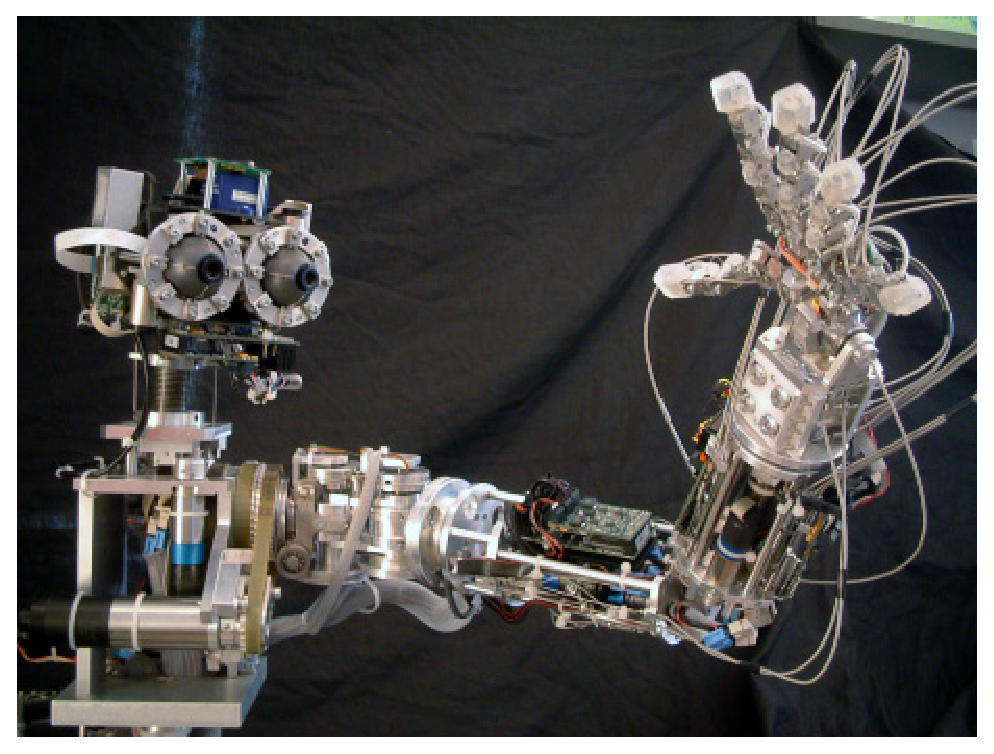
\includegraphics[width=7cm]{../robustIntelligentSystems07/James1.eps}
		\caption{James, a humanoid upper torso.}
	\label{fig:James1}
\end{figure}

The big advantage of modular control relies in the possibility
of combining previous experience to handle new situations. It was shown
that this advantage requires to interpret the current
context as the combination of previously experienced contexts.
In order to perform such an interpretation, it becomes crucial the 
use of sensors (primarily vision and touch) capable of extracting 
from the environment context related information. Therefore, the
implementation of these ideas seems to fit perfectly within
the field of humanoid robotics (see figure \ref{fig:James1}). 

\section*{Acknowledgements}

The work presented in this paper has been supported by the project
\textsc{Robot Cub} (IST-2004-004370) and by the project
\textsc{Neurobotics} (IST-2003-511492). Both projects are funded by
the European Union through the Sixth Framework Programme for
Research and Technological Development (FP6).

\appendix

\section{Minimum Number of Motion Primitives} \label{Sec:MinNumPrimitives}

\subsection{Lower Bound on the Number of Elementary Controls} \label{Sec:LowerBound}

In this Section it is proved that any given solution of Prb.
\ref{Prb:ElemContrSynth} is composed by at least $n$
elementary controls, i.e. $K \geq n$. Before giving the main
result, it is important to recall the following lemma, claiming the 
injectivity of the function $\lambda$. In the following the set of reachable
states is denoted $\mathcal X \subseteq \mathbb R^n$.

\begin{lemma} \label{Lem:OneToOne}
Let $\{\Phi^1$, $\dots$, $\Phi^K\}$ and $\lambda : \mathcal X
\rightarrow \mathbb R^K$ be a solution to
Problem \ref{Prb:ElemContrSynth}. Then $\lambda(\x_f)$ is injective.
\end{lemma}

\ProofBegin Suppose by contradiction that there exist 
$\mathbf x_f^1$ and $\mathbf x_f^2$ such
that $\mathbf x_f^1 \neq \mathbf x_f^2$ but $\lambda(\mathbf
x_f^1) = \lambda(\mathbf x_f^2)$. Define:
\begin{eqnarray}
\mathbf u^1 & \triangleq & \sum_{k=1}^K \lambda_k(\mathbf
x_f^1) \Phi^k(\mathbf x), \\ \mathbf u^2 & \triangleq &
\sum_{k=1}^K \lambda_k(\mathbf x_f^2) \Phi^k(\mathbf x).
\end{eqnarray}
Under the given assumption $\mathbf u^1 = \mathbf u^2$, but this
contradicts the fact that $\mathbf u^1$ drives the system to 
$\mathbf x_f^1 \neq \mathbf x_f^2$. By contradiction, this proves 
that $\lambda$ is injective. \ProofEnd

\begin{fact} \label{Pro:LowerBound}
Let $\{\Phi^1$, $\dots$, $\Phi^K\}$ and $\lambda : \mathcal X
\rightarrow \mathbb R^K$ be a solution to Problem
\ref{Prb:ElemContrSynth}. Then $K \geq n$.
\end{fact}

\ProofBegin Using Lemma \ref{Lem:OneToOne}, we have that
$\lambda(\cdot)$ is a continuously differentiable injective
function from an open subset of $\mathbb R^n$ to $\mathbb R^K$. It
can be proved that this implies $K \geq n$ (see \cite{Boothby} for 
details). \ProofEnd
%%%%%%%%%%%%%%%%%%%%%%%%%%%%%%%%%%%%%%%%%%%%%%%%%%%%%%%%%%%%%%%%%%%%%%%%%%


%%%%%%%%%%%%%%%%%%%%%%%%%%%%%%%%%%%%%%%%%%%%%%%%%%%%%%%%%%%%%%%%%%%%%%%%%%

\subsection{Minimum number of elementary controls} \label{Sec:MinNumPrimitivesNonLin}

It was shown that we need at least $n$ 
primitives to preserve controllability. It is here proved that $n$ are not
sufficient under suitable assumptions. Let's consider an affine nonlinear system 
of type \eqref{Eq:NonLinMod}. Let $\{\Phi^1$, $\dots$, $\Phi^K\}$, $\lambda 
: \mathcal X \rightarrow \mathbb R^K$ be a solution to Problem 
\ref{Prb:ElemContrSynth}. Moreover, define $\mathcal
X_{\mbox{eq}} \subset \mathcal X$ to be the set of equilibrium
points with $\mathbf u = 0$, i.e. $\mathbf x_f \in \mathcal
X_{\mbox{eq}}$ if and only if $f(\mathbf x_f) = 0$. The proof of
the main result requires the following additional assumption.
\\
\\
\textbf{(HP)}. $\mathcal X_{\mbox{eq}} \neq \emptyset$ and
$\forall \x_f \in \mathcal X_{\mbox{eq}}$ the solution of the
following differential equation:
\begin{eqnarray}
\left\{ \begin{array} {l} \mathbf {\dot x} = f (\mathbf x) +
g(\mathbf x) \sum_{k=1}^K \lambda_k(\x_f) \Phi^k(\x, t)\\
\mathbf x(0) = \x_f
\end{array} \right. .
\end{eqnarray}
is $\mathbf x(t) \equiv \mathbf x_f$, $\forall t \in [0, T]$.
Basically, this is equivalent to requiring that if we start at an
equilibrium point and we want to reach the same equilibrium point,
then this is accomplished leaving the system in the same position
for the entire time interval.

\begin{theorem} \label{Th:MinNumPrimNonLin}
Let $\{\Phi^1, \dots, \Phi^K\}$, $\lambda: \mathcal X \rightarrow
\mathbb R^K$ be a solution to Problem
\ref{Prb:ElemContrSynth} with dynamics given by
(\ref{Eq:NonLinMod}). Moreover, assume that for the
given solution, (HP) holds. Then $K \geq n+1$.
\end{theorem}

\ProofBegin Suppose by contradiction that $K < n + 1$. Since it was
shown that $K \geq n$, only one possibility is left out:
$K=n$. Define:
\begin{eqnarray}
\varPhi(\x, t) \triangleq \begin{bmatrix} \Phi^1(\x, t) & \dots &
\Phi^n(\x, t) \end{bmatrix} \qquad \lambda(\x_f) \triangleq \begin{bmatrix} \lambda_1(\x_f) & \dots &
\lambda_n(\x_f) \end{bmatrix}^\top,
\end{eqnarray}
so that the following holds:
\begin{eqnarray}
\sum_{k=1}^n \lambda_k(\x_f) \Phi^k(\x, t) = \varPhi(\x, t)
\lambda(\x_f).
\end{eqnarray}
Since the proposed primitives solve Prb.
\ref{Prb:ElemContrSynth}, the following system:
\begin{eqnarray} \label{Eq:BasicSystemControlSimply}
\left\{ \begin{array} {l} \mathbf {\dot x} = f (\mathbf x) +
g(\mathbf x) \varPhi(\x, t) \lambda(\x_f) \\
\mathbf x(0) = \x_0 \in \mathcal X
\end{array} \right. ,
\end{eqnarray}
converges to $\mathbf x_f$, $\forall \x_f \in \mathcal X$
regardless of the initial condition. Consider $\x_f \in \mathcal
X_{\mbox{eq}}$ and $\mathbf x(0) = \x_f$. Using (HP) in
(\ref{Eq:BasicSystemControlSimply}), we get:
\begin{eqnarray} \label{Eq:IdentNullControlAct}
g(\mathbf x_f) \varPhi(\x_f, t) \lambda(\x_f) = 0, \quad \quad
\forall t \in [0, T].
\end{eqnarray}
Now, let's use the fact that the image of $\mathcal X$ under
$\lambda: \mathcal X \rightarrow \mathbb R^n$ is an open set in $\mathbb R^n$.
This is consequence of the fact that $\lambda$ is injective and
$\mathcal C^1(\mathcal X)$ with $\mathcal X$ open (see \cite{Boothby} for details). If
$\mbox{Im}_\lambda(\mathcal X)$ is open and $\lambda(\x_f) \in
\mbox{Im}_\lambda(\mathcal X)$, we can always find $\mu \neq 1$
such that $\mu \lambda(\x_f) \in \mbox{Im}_\lambda(\mathcal X)$;
we only need to take $|1-\mu|$ small enough. Therefore, there
always exists $\tilde \x_f \in \mathcal X$, such that
$\lambda(\tilde \x_f) = \mu \lambda(\x_f)$. According to the given
hypothesis, the following system:
\begin{eqnarray} \label{Eq:ControlledSysTilde}
\left\{ \begin{array} {l} \mathbf {\dot x} = f (\mathbf x) +
g(\mathbf x) \varPhi(\x, t) \lambda(\tilde \x_f) \\
\mathbf x(0) = \x_0 \in \mathcal X
\end{array} \right. ,
\end{eqnarray}
should converge to $\tilde \x_f$ regardless of the initial
condition. However, take $\mathbf x_0 = \x_f$, and observe that
the corresponding trajectory is given by $\x(t) \equiv \x_f$,
$\forall t \in [0, T]$ since we have:
\begin{eqnarray*}
\mathbf {\dot x} = f (\mathbf x_f) + g(\mathbf x_f) \varPhi(\x_f,
t) \lambda(\tilde \x_f) = \mu g(\mathbf x_f) \varPhi(\x_f, t)
\lambda(\x_f) \stackrel{
(\ref{Eq:IdentNullControlAct})}{=} 0 \quad \forall t \in
[0, T].
\end{eqnarray*}
Therefore, we have found an initial condition for
(\ref{Eq:ControlledSysTilde}) that is not driven to $\tilde
\x_f$. This is in contradiction with our hypothesis.\ProofEnd
%%%%%%%%%%%%%%%%%%%%%%%%%%%%%%%%%%%%%%%%%%%%%%%%%%%%%%%%%%%%%%%%%%%%%%%%%%

\bibliographystyle{alpha}
\bibliography{author}


%%%%%%%%%%%%%%%%%%%%%%%%%%%%%%%%%%%%%%%%%%%%%%%%%%%%%%%%%%%%%%%%%%%%%%

%%%%%%%%%%%%%%%%%%%%%%%%%%%%%%%%%%%%%%%%%%%%%%%%%%%%%%%%%%%%%%%%%%%%%%

%\printindex
\end{document}
